\documentclass[submitting]{nst}

\usepackage{subfigure,dcolumn}
\usepackage{epstopdf}
\usepackage{mhchem}
\usepackage{upgreek}
\usepackage{subfigure}
\usepackage{physics}
\usepackage{listings}
\usepackage{dcolumn}

\begin{document}

\title{Features of dual-purpose structure for heavy ion and light particles}
%\thanks{Supported by the Program for Science \& Technology Innovation Talents in Universities of Henan Province (No.~13HASTIT046) and the Young Teacher Project in Henan Normal University}

\author{Kolokolchikov S. D.}
\email[Corresponding author, ]{sergey.bell13@gmail.com}
\affiliation{Institute for Nuclear Research of the Russian Academy of Sciences, Moscow 117312, Russia}

\author{Senichev Yu. V.}
\affiliation{Institute for Nuclear Research of the Russian Academy of Sciences, Moscow 117312, Russia}

\author{Aksentyev A. E.}
\affiliation{Institute for Nuclear Research of the Russian Academy of Sciences, Moscow 117312, Russia}
\affiliation{National Research Nuclear University MEPhI, Moscow 115409, Russia}

\author{Melnikov A. A.}
\affiliation{Institute for Nuclear Research of the Russian Academy of Sciences, Moscow 117312, Russia}
\affiliation{Landau Institute for Theoretical Physics, Chernogolovka 142432, Russia}


\begin{abstract}
The different charge-to-mass ratio is essential in magneto-optics design. To achieve high luminosity sufficient beam lifetime must be guaranteed. Transition energy crossing must also be solved. The NICA collider will be used for both collider experiments with heavy ions and light polarized nuclei.
\end{abstract}

\keywords{Transition energy, Intrabeam scattering, Stochastic cooling, Resonant structure, Dual-purpose structure}

\maketitle

\section{Introduction}\label{sec.I}
\par Regardless of the purpose of the synchrotron, always in the case of two modes, when multiply charged heavy particles and one or two charged light particles are accelerated, the problem arises of what the magneto-optical structure should look like to satisfy all the conditions of stable motion for both types of particles. Obviously, compared to light particles, multiply charged particles have a prevailing heating effect due to intra-beam scattering, and light particles have a greater chance of crossing through transition energy. All these effects are of great importance for colliders, where luminosity plays a decisive role. When developing a structure that meets all the requirements for differently charged particles, it is fundamentally important to have a retunable structure without introducing design differences. We called such a structure -- dual-purpose or simple, dual.
\par In NICA complex the dual magneto-optical structure opens up the prospect of accelerating both heavy ions, such as gold, and light particles like protons and deuterons. The design of this structure requires a different approach due to the varying charge-to-mass ratios involved.
\section{Light particles}\label{sec.II}
In a classical regular structure, the transition energy is approximately equal to the betatron tune $\gamma_{\text{tr}}\simeq\nu_{\text{s}}$ \cite{b1}. For the same magnetic rigidity $B\rho$, the maximum energy for light particles is greater than for heavy ions due to their charge-to-mass ratio. This means that a heavy-ion structure optimized for operating up to a certain transition energy would require overcoming that energy in order to operate with light particles. For this reason, a structure with varying transition energy can be considered.
\subsection{Transition energy}
\par In general, the transition energy is determined by the momentum compaction factor
\begin{equation}
\alpha=\frac{1}{{\gamma_{\text{tr}}}^2}=\frac{1}{C}\int_{0}^{C}{\frac{D\left(s\right)}{\rho\left(s\right)}ds}
\end{equation}
\noindent where $C$ -- orbit length, $D(s)$ -- dispersion function, $\rho(s)$ -- radius of orbit curvature. It is a characteristic of the structure and remains constant regardless of the particle type. In the first order the slip-factor $\eta=\eta_0=1/\gamma_{\text{tr}}^2-1/\gamma^2$, and thus the frequency of synchrotron oscillations $\omega_{\text{s}}\ \sim \eta$ tends to zero when the beam energy approaches the transition value. In this case, the adiabaticity of the longitudinal phase motion is violated, which leads to instabilities, as well as the influence of nonlinear effect higher orders of momentum spread $\delta$. The introduction of modulation into the $D\left(s\right)$ or $\rho\left(s\right)$, function leads to variations in the momentum compaction factor and, consequently, the transition energy.
\subsection{Superperiodic modulation}
The equation for the dispersion function with biperiodic variable focusing \cite{b2}	
\begin{equation}
\dv[2]{D}{s}+\left[K(s)+\varepsilon k(s)\right]D=\frac{1}{\rho(s)},
\label{eq:disp_eq}
\end{equation}
\noindent where $K\left(s\right)=\frac{e}{p}G\left(s\right)$, $\varepsilon k\left(s\right)=\frac{e}{p}\Delta G\left(s\right)$, $G\left(s\right)$ -- gradient of magneto-optical lenses, $\Delta G\left(s\right)$ -- superperiodic gradient modulation. Here is considered an additional perturbation to regular one $\varepsilon k\left(s\right)=\sum_{k=0}^{\infty}g_k\cos(k\phi)$, where $g_k$ -- $k$-th harmonic of the gradient modulation in the Fourier series expansion of the function. The solution for momentum compaction factor as follows for only gradient modulation
\begin{equation}
\begin{aligned}
\alpha_{\text{s}}= & \frac{1}{\nu^2}\left\{1+\frac{1}{4(1-k S / \nu)}\left(\frac{\bar{R}}{\nu}\right)^4 \frac{g_k^2}{\left[1-(1-k S / \nu)^2\right]^2}\right\}.
\end{aligned}
\label{eq:alpha_gradient}
\end{equation}
\noindent where ${\overline{R}}_{\text{arc}}$ -- the average value of the curvature, $\nu_x$ -- betatron tune in horizontal plane on arc, $S$ -- number of superperiods per arc length. Eq. (\ref{eq:alpha_gradient}) considered without introducing curvature modulation due to the possibility of introducing a variation of transition energy into a stationary lattice. To raise the transition energy, it is necessary to reduce $\alpha_{\text{s}}=1/\gamma_{\text{tr}}^{\text{arc}}$, this means that the expression under the sum sign must be negative, this is realizable under the condition $kS/\nu_{x, \text{arc}}>1$.
\par First harmonic $k=1$ has a dominant influence the condition is implemented for $S=4, \nu_{x, \text{arc}}=3$. Fig. \ref{fig:pure_resonant} shows 12 FODO cells per arc, 3 FODO cells are combined into one superperiod \cite{b3}. Thus, due to the tune of betatron tune a multiple of $2\pi$, the arc has the properties of a first-order achromat. For structure with the missing magnet technique introduced for one reason or another it can be also implemented (Fig. \ref{fig:resonant}), but need to suppress dispersion at the edge of arc \cite{b4}.
\begin{figure}[!htb]
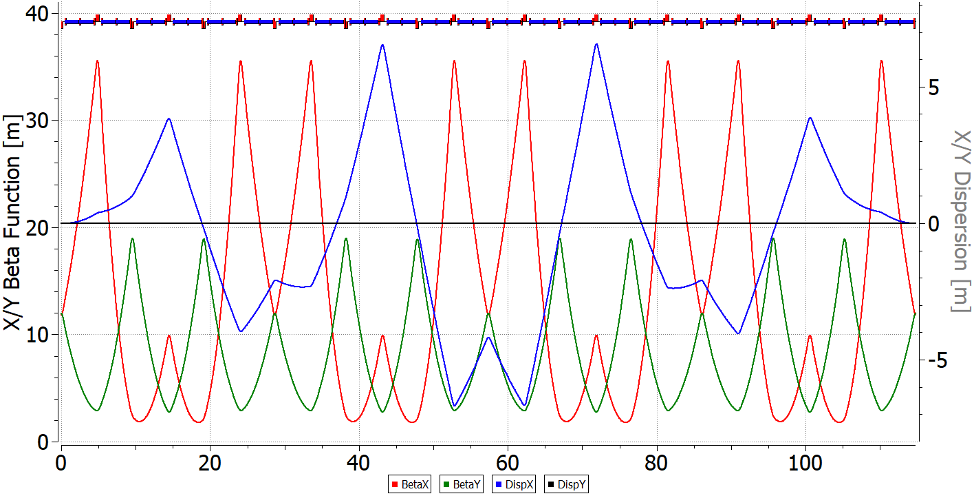
\includegraphics[width=\hsize]{fig1_pure_resonant}
\caption{(Color online) "Resonant" magneto-optic structure with dispersion modulation and increased transition energy.}
\label{fig:pure_resonant}
\end{figure}
\begin{figure}[!htb]
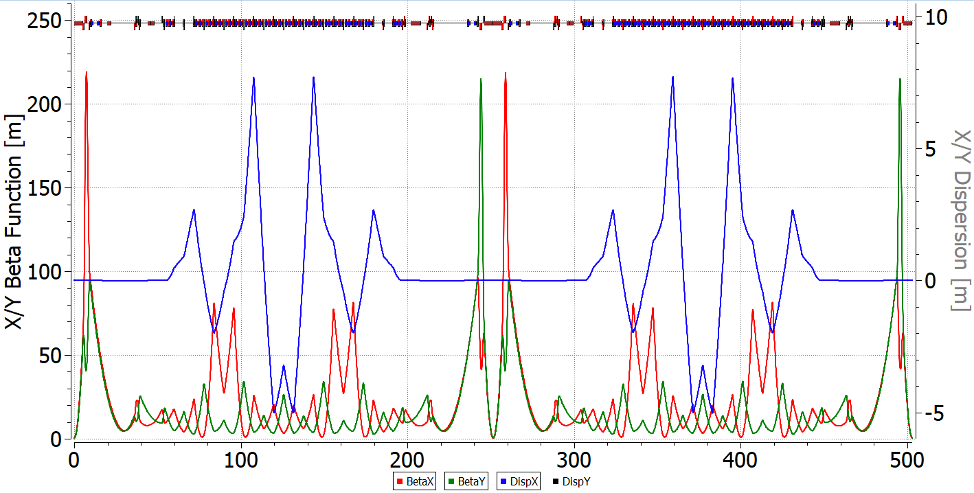
\includegraphics[width=\hsize]{fig2_resonant.png}
\caption{(Color online) "Resonant" NICA magneto-optic adapted structure with increased transition energy and missing magnet.}
\label{fig:resonant}
\end{figure}
\section{Heavy ion mode}\label{sec.III}
The lifetime of the beam luminosity in a collider experiment is achieved through the reduction of intra-beam scattering effects, coupled with the application of stochastic and electron beam cooling techniques. This approach assumes particular significance when dealing with high-intensity ion beams. The temporal evolution of emittance and momentum spread in the presence of cooling processes is governed by a set of equations
\begin{equation}
\begin{aligned}
& \dv{\varepsilon}{t} =\underbrace{-\frac{1}{\tau_{\text{tr}}} \cdot \varepsilon}_{\text {cooling}}+\underbrace{\left(\dv{\varepsilon}{t}\right)_{\text{IBS}}}_{\text {heating}} \\
& \dv{\delta^2}{t} =\underbrace{-\frac{1}{\tau_{\text {long }}} \cdot \delta^2}_{\text {cooling}}+\underbrace{\left(\dv{\delta^2}{t}\right)_{\text {IBS}}}_{\text {heating}} \\
&
\end{aligned}
\end{equation}
\noindent where $\varepsilon$ -- transverse emittance, $\tau_{\text{tr}}$ -- transverse cooling time, $\delta=\frac{\Delta p}{p}$ -- momentum spread, $\tau_{\text{long}}$ -- longitudinal cooling time.
\noindent For time-independent, stationary values, the time derivatives become zero, then
\begin{equation}
\begin{aligned}
& \varepsilon_{\textrm{st}}=\left.\tau_{\textrm{tr}} \cdot\left(\dv{\varepsilon}{t}\right)_{\textrm{IBS}}\right|_{\varepsilon=\varepsilon_{\textrm{st}}} \\
& \delta_{\text{st}}^2=\left.\tau_{\text{long}} \cdot\left(\dv{\delta^2}{t}\right)_{\text{IBS}}\right|_{\delta^2=\delta_{\textrm{st}}^2}
\end{aligned}
\end{equation}
The benchmark for evaluating the effectiveness of a cooling technique can be determined by comparing the timescales of stochastic or electron cooling processes to the beam lifetime due to IBS over the entire energy spectrum.
\subsection{Stochastic cooling}
\par Let's consider stochastic cooling using the approximate theory developed by D.Mohl \cite{b5, b6}. Based on his main findings, the cooling rate can be determined using the following expression
\begin{equation}
\frac{1}{\tau_{\textrm{tr, l}}}=\frac{W}{N}[\underbrace{2 g \cos \theta\left(1-1 / M_{\textrm{pk}}^2\right)}_{\begin{array}{c}
\text { coherent } \\
\text { effect(cooling) }
\end{array}}-\underbrace{g^2\left(M_{\textrm{kp}}+U\right)}_{\begin{array}{c}
\text { incoherent } \\
\text { effect(heating) }
\end{array}}]
\label{eq:stochastic_rate}
\end{equation}	
\noindent where $W=f_{\text{max}}-f_{\text{min}}$ -- system bandwidth, $N$ -- effective number of particles, recalculated based on the ratio of orbit length to the beam length, considering its distribution, $g$ -- fraction of observed sample error corrected per turn, $U$ -- the ratio of noise to signal, $M_{\text{pk}}$, $M_{\text{kp}}$ -- mixing factors between the pickup-kicker and the kicker-pickup, respectively. Eq. (\ref{eq:stochastic_rate}) in the absence of noise at $g=g_0={\frac{1-{M_{\text{pk}}}^2}{M_{\text{kp}}}}$ reaches the maximum
\begin{equation}
\begin{aligned}
& \frac{1}{\tau_{\textrm{tr}}}=\frac{W}{N} \frac{\left(1-1 / M_{\textrm{pk}}^2\right)^2}{M_{\textrm{kp}}} \\
& \frac{1}{\tau_{\textrm{l}}}=2 \frac{W}{N} \frac{\left(1-1 / M_{\textrm{pk}}{ }^2\right)^2}{M_{\textrm{kp}}}
\end{aligned} 
\label{eq:cooling_rate}
\end{equation}
\noindent The mixing coefficients are defined as
\begin{equation}
\begin{aligned}
M_{\textrm{pk}} & =\frac{1}{2\left(f_{\max }+f_{\min }\right) \eta_{\textrm{pk}} T_{\textrm{pk}} \frac{\Delta p}{p}}, \\
M_{\textrm{kp}} & =\frac{1}{2\left(f_{\max }-f_{\min }\right) \eta_{\textrm{kp}} T_{\textrm{kp}} \frac{\Delta p}{p}}
\end{aligned}
\label{eq:mixing_coeff}
\end{equation}
\noindent where $\eta_{\text{pk}}T_{\text{pk}}\delta$, $\eta_{\text{kp}}T_{\text{kp}}\delta$ -- relative particle displacement times (mixing),  $\eta_{\text{pk}}$, $\eta_{\text{kp}}$ -- slip-factor, as a first approximation $\eta_{\text{pk}}=\alpha_{\text{pk}}-1/\gamma^2$, $\eta_{\text{kp}}=\alpha_{\text{kp}}-1/\gamma^2$, $\alpha_{\text{pk}}$, $\alpha_{\text{kp}}$ -- first-order of local momentum compaction factors, $T_{\text{pk}}$, $T_{\text{kp}}$ -- the absolute times between the pickup-kicker and kicker-pickup, respectively. The stochastic cooling times of Eq. (\ref{eq:cooling_rate}) depend on the ratio of the effective particle density to the cooling system bandwidth and the properties of magneto-optics, local momentum compaction factors $\alpha_{\text{pk}}$, $\alpha_{\text{kp}}$.

\par The maximum value of the frequency band is determined by the requirement that the "Schottky" beam bands do not overlap. In the simplest case, this can be expressed:

\begin{equation}
f_{\textrm{max}}<\frac{1}{\eta_{\textrm{pk}}T_{\textrm{pk}}\frac{\Delta p}{p}}
\end{equation}

\noindent thus, a mixing factor $M_{\text{pk}}>1$. Otherwise, the cooling efficiency becomes zero. Thus, for a given number of particles, it is desirable to achieve the highest possible frequency band. From an electron perspective, modern technologies allow for the implementation of a $10$ GHz frequency band \cite{b7}, however, its use is not always feasible due to the large magnitude of the slip-factor $\eta_{\text{pk}}$ and momentum spread $\delta$.

\par Eq. (\ref{eq:stochastic_rate}) has been derived for coasting beam. Particle density for a single harmonic RF resonator is described by a Gaussian distribution

\begin{equation}
\rho(s)=\frac{N_{\textrm{bunch}}}{\sigma_{\textrm{bunch}}\sqrt{2\pi}}\cdot e^{-\frac{s^2}{2\sigma_{\textrm{bunch}}^2}}\ \ \ 
\end{equation}	

\noindent where $s$ – the distance from the beam center, $\sigma_{\text{bunch}}$ – the dispersion of the particle distribution, and $N_{\text{bunch}}$ – the number of particles. Assuming that cooling is at its minimum at the center ($s=0$), the effective particle number at orbit length $C_{\text{orb}}$ can be calculated as follows:

\begin{equation}
N=\frac{N_{\textrm{bunch}}}{{4\sigma}_{\textrm{bunch}}}\cdot C_{\textrm{orb}}
\end{equation}

\noindent For a beam generated by a multiharmonic barrier-type RF system, so-called "Barrier Bucket", the particles distribution in the beam can be considered approximately uniform along its entire length. The effective particles number is determined by a simple ratio of the beam length to the total orbit length:

\noindent To summarize, the effective value of particles depends on their distribution and is determined by their form-factor $F_{\text{bunch}}=\sqrt{2\pi}\divisionsymbol4$

\begin{equation}
N=N_{\textrm{bunch}}\cdot\frac{C_{\textrm{orb}}}{F_{\textrm{bunch}}\cdot\sigma_{\textrm{bunch}}}
\end{equation}

As example let us consider the case of NICA with maximal form-factor $F_{\text{bunch}}=4$ with $C_{\text{orb}}=503.04$ m, $\sigma_{\text{bunch}}=0.6$ m, $N_{\text{bunch}}=2.2\cdot{10}^9$. Considering the accumulated FNAL \cite{b8} experience, quite realistic values for the frequency band are $f_{\text{max}}=8$ GHz and $f_{\text{min}}=2$ GHz. For NICA $f_{\text{max}}=4$ GHz and $f_{\text{min}}=2$ GHz. With these parameters, the maximum achievable cooling rate is $1/\tau_{\text{tr}}=1/230$ $\text{s}^{-1}$.


\par Based on Eq. (\ref{eq:mixing_coeff}), it is evident that asymptotic growth may occur in two scenarios:
\begin{enumerate}
\item slip-factor approaches the value $\eta\rightarrow\frac{1}{2\left(f_{\text{max}}+f_{\text{min}}\right)T_{\text{pk}}\delta}$, the beam Schottky spectrum becomes continuous and $M_{\text{pk}}\rightarrow1$;
\item slip-factor approaches zero, mixing between the kicker to the pickup does not occur and $M_{\text{kp}}\rightarrow\infty$.
\end{enumerate}
\noindent The efficiency of stochastic cooling depends on the properties of magneto-optical structure. In classical “regular” structures, transition energy is acquired through the horizontal frequency $\gamma_{\text{tr}}\approx\nu_x$ and slip-factor $\eta=1/\gamma_{\text{tr}}^2-1/\gamma^2$ can achieve zero. To avoid asymptotic growth, it is necessary to vary the slip-factor which means $\gamma_{\text{tr}}$. This is possible in “resonant” structure, where transition energy can be increased or even reach complex value. In more exotic case, can be used “combined” structure then $\eta_{\text{pk}}$ (pickup-kicker) with real transition energy at one arc
\begin{equation}
\eta_{\textrm{pk}}=1/\gamma_{\textrm{tr}}^2-1/\gamma^2
\label{eq:eta_pk}
\end{equation}
\noindent compensated by $\eta_{\text{kp}}$ (kicker-pickup) with complex transition energy at another

\begin{equation}
\eta_{\textrm{kp}}=-1/\gamma_{\textrm{tr}}^2-1/\gamma^2
\label{eq:eta_kp}
\end{equation}
\noindent for the whole ring. Such structure achieves the required ratio of mixing factors for a maximum cooling rate close to ideal \cite{b9}. Let us delve deeper declared structures in more detail.
\par The behaviour of the $\beta$-functions and $D$ the dispersion across the entire “regular” ring illustrates at Fig. \ref{fig:regular}. The straight sections, which remain constant in all structures, are essential for analyzing of the resonant characteristics of the entire structure. Their arrangement does not affect the intra-beam scattering and transition energy. To suppress dispersion in the “regular” structure, ‘missing magnets’ technic implemented on both sides of the arc.
\noindent The “resonant” structure is based on the principle of resonant modulation of the dispersion function and can be obtained from a "regular" one by introducing additional family of focusing quadrupoles. To suppress dispersion can be used either two edge focusing quadrupoles on both sides of the arc or only two families of focusing quadrupoles on the arc, when an integer number of betatron oscillations is reached.
\begin{figure}[!htb]
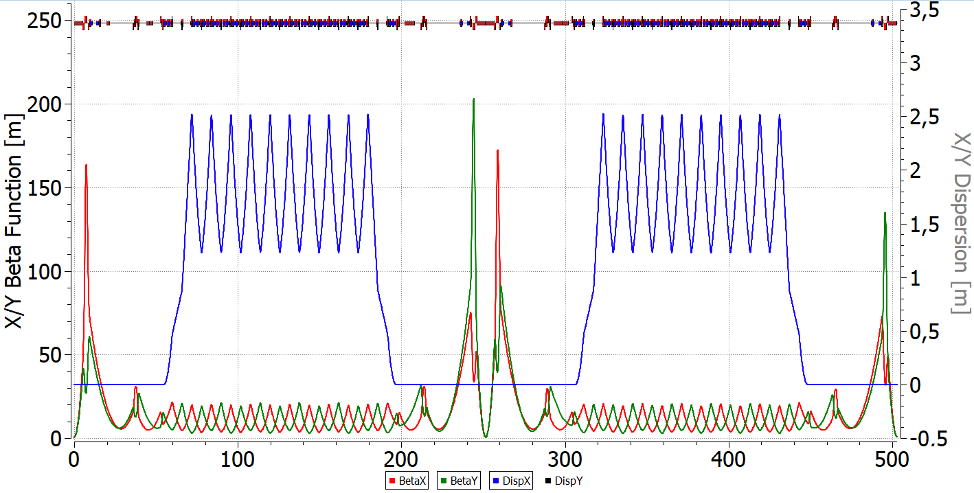
\includegraphics[width=\hsize]{fig3_regular.png}
\caption{(Color online) “Regular” FODO NICA magneto-optic structure with missing magnets.}
\label{fig:regular}
\end{figure}

\noindent The case of a “combined” structure, one arc operates in a regular mode, while the other employs resonant modulation (Fig. \ref{fig:combined}). Such choice is based on the principle of compensation, as described by Eqs. \ref{eq:eta_pk}, \ref{eq:eta_kp}, which requires a greater modulation depth of the quadrupoles than in purely "resonant" structure with increased transition energy.
\begin{figure}[!htb]
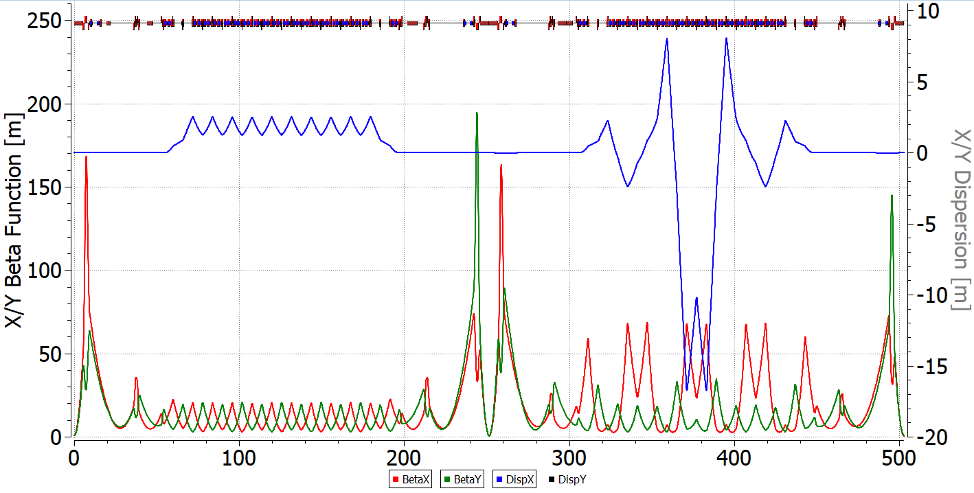
\includegraphics[width=\hsize]{fig4_combined.png}
\caption{(Color online) "Combined" NICA magneto-optic structure with real and complex transition energies in arcs.}
\label{fig:combined}
\end{figure}	
\noindent As illustrated in Fig. \ref{fig:sc}, "resonant" optics with increased transition energy, the second asymptotic is at higher energy compared to the “regular” structure. In “combined” magneto-optics, the cooling efficiency is closer to the ideal value in a large energy range from $2.5$ to $4.5$ GeV, while in “regular” optics the cooling rate is almost two times lower at the most optimal point $\sim3$ GeV. This behaviour is explained by absence of the second point of asymptotic growth.
\begin{figure}[!htb]
\centering
\subfigure[] {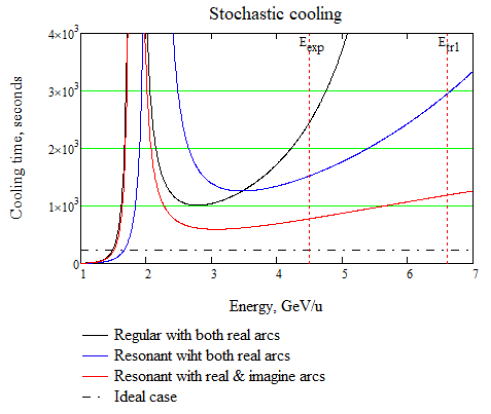
\includegraphics[width=0.235\textwidth]{fig5.1_SC.png}}
\subfigure[] {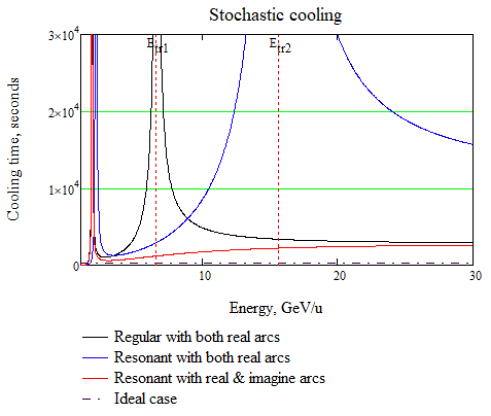
\includegraphics[width=0.235\textwidth]{fig5.2_SC_wide.png}}
\caption{(Color online) The dependence of stochastic cooling time on the energy for various structures. Energy range (a) $1-7$, (b) 0-30 GeV per nuclon.}
\label{fig:sc}
\end{figure}	
\subsection{Intrabeam Scattering}
\par Intra-beam scattering represents a fundamental limitation on the beam lifetime in the collider. Consequently, the selection of an appropriate cooling technique hinges on comparing its characteristic time scales with the rate at which the beam is heated due to intra-beam scattering. This is derived from the fundamental principles governing this process
\begin{equation}
\begin{aligned}
\frac{1}{\tau_{\textrm{IBS}}}=\frac{\sqrt\pi}{4}\frac{cZ^2r_p^2L_C}{A}&\cdot\frac{N}{C_{\mathrm{orb\ }}}\cdot\frac{\left\langle\beta_x\right\rangle}{\beta^3\gamma^3\varepsilon_x^{5/2}\left\langle\sqrt{\beta_x}\right\rangle}\times\\
&\times\left(\left\langle\frac{D_x^2+{\dot{D}}_x^2}{\beta_x^2}\right\rangle-\frac{1}{\gamma^2}\right)
\end{aligned}
\label{eq:ibs}
\end{equation}

\begin{figure}[!htb]
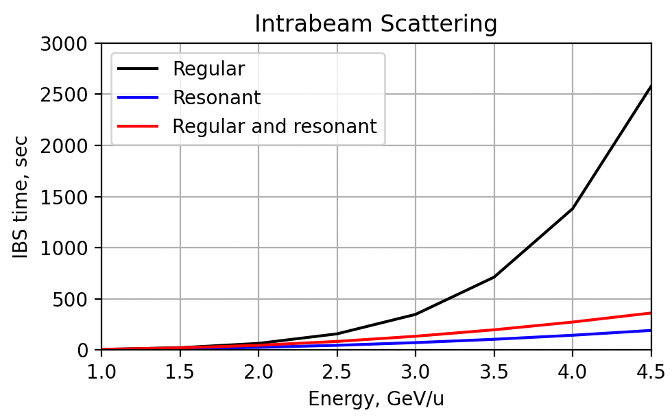
\includegraphics[width=\hsize]{fig6_IBS}
\caption{(Color online) The dependence of the beam lifetime due to intra-beam scattering in “regular”, "resonant" and “combined” structures on the beam energy for heavy ion beam.}
\label{fig:ibs}
\end{figure}

\noindent Unlike stochastic cooling, the IBS rate increases as decreasing energy $1/\gamma^3$. In addition, the expression in parentheses is proportional to the slip-factor $\eta$. Therefore, it should be expected that in optics with a value $\eta$ close to zero, the heating rate should decrease. Fig. \ref{fig:ibs} shows the dependences of the heating time constant in the three above-mentioned structures calculated using MADX programs \cite{b10} for the parameters of the heavy ion beam ${_{79}^{197}}\text{Au}$ of the NICA collider with maximum luminosity ${10}^{27}\ {\text{sm}}^{-2}\text{s}^{-1}$. In the context of light nuclei, such as protons and deuterons, the IBS time experiences a significant increase as the charge decreases. Consequently, the issue of intra-beam scattering becomes critical for heavy-ion beam.
From the comparison of the IBS lifetime with the cooling time it can be concluded that in a regular structure, stochastic cooling is able to balance intra-beam scattering in the energy range $W\geq4.5\ \text{GeV}$. In order to apply stochastic cooling over the entire energy range, it is obvious that we must sacrifice the luminosity of the beam at low energies by increasing the emittance. In resonant structures, the IBS time is notably reduced. This is explained by the fact that the structure has a greater ratio $\left\langle\frac{D_x^2+{\dot{D}}_x^2}{\beta_x^2}\right\rangle$ between the dispersion and the beam $\beta$-function than in the case of a regular. Thus, for the case of heavy ions, the configuration should be regular and minimally modulated. Electron cooling is used in the regular structure to cool the beam lower $4.5$ GeV \cite{b11, b12}.

\begin{table}[!htb]
\caption{Main parameters of structures.}
\label{tab:dual}
\begin{tabular*}{8cm} {@{\extracolsep{\fill} } lccc}
\toprule
Structure & Regular & Resonant & Combined \\
\midrule
Energy, GeV per nuclon & 4.5 & 12.6 & 12.6 \\
Transition energy $\gamma_{\text{tr}}$  & 7 & 15 & $i50$ \\
Modulation depth & -- & 25\% & 45\% \\
Stochastic cooling at $4.5$ GeV, s & 2500 & 1500 & 800 \\
IBS time at $4.5$ GeV, s & 2500 & 400 & 250 \\
\bottomrule
\end{tabular*}
\end{table}

\section{Summary} \label{sec.IV}

\par The dual magneto-optical structure is proposed for accelerating both heavy ion and light particle beams, exemplified by the NICA facility. For light particles, due to charge-to-mass ratio, experiment energy can rise more than transition energy of the lattice, which is optimal for heavy ions. Using dispersion modulation, transition energy increases or even reaches a complex value in a “resonant” magneto-optic structure. However, due to modulation of $\beta$-function and $D$ dispersion, the time of intra-beam scattering decreases, which is crucial for multiply charged heavy particles. For this reason, a “regular” magneto-optic structure with minimally modulated dispersion and $\beta$-function is optimal in the heavy-ion mode. Despite the fact that stochastic cooling in “regular” structures is significantly weaker than in “resonant” and “combined’ ones, it can compensate IBS effect.
\par No special changes are required to convert the “regular” structure into a “resonant” one. It is enough only to introduce a separate family of quadrupoles

\begin{thebibliography} {99}

\bibitem{b1}	Lee, S.-Y., Accelerator Physics (Fourth Edition), {\it World Scientific Publishing Company}, 2018 \href{https://doi.org/10.1142/11111}{doi:10.1142/11111}
\bibitem{b2}	Senichev, Y.V., Chechenin, A.N. Theory of “Resonant” lattices for synchrotrons with negative momentum compaction factor. {\it J. Exp. Theor. Phys.} {\bf 105}, 988–997 (2007). \href{https://doi.org/10.1134/S1063776107110118}{doi:10.1134/S1063776107110118}
\bibitem{b3}	Senichev, Y.V., Chechenin, A.N. Construction of “resonant” magneto-optical lattices with controlled momentum compaction factor. {\it J. Exp. Theor. Phys.} {\bf 105}, 1141–1156 (2007). \href{https://doi.org/10.1134/S1063776107120060}{doi:10.1134/S1063776107120060}
\bibitem{b4}	Kolokolchikov, S.D., Senichev, Y.V. Magneto-Optical Structure of the NICA Collider with High Transition Energy, {\it Phys. Atom. Nuclei} {\bf 84}, 1734–1742 (2021). \href{https://doi.org/10.1134/S1063778821100185}{doi:10.1134/S1063778821100185}
\bibitem{b5}	D. Möhl, G. Petrucci, L. Thorndahl and S. van der Meer, {\it Phys. Rep.} {\bf 58} (1980) 75 \href{https://doi.org/10.1016/0370-1573(80)90140-4}{doi:10.1016/0370-1573(80)90140-4}
\bibitem{b6}	D. Möhl, {\it Nuclear Instruments and Methods in Physics Research} {\bf A 391} (1997), 164-171 \href{https://doi.org/10.1016/S0168-9002(97)00360-4}{doi:10.1016/S0168-9002(97)00360-4}
\bibitem{b7}	F.Caspers, D. Möhl , Stochastic Cooling in Hadron Colliders, {\it Proc. of XVII International Conference High Energy Accelerators}, 1998, Dubna \href{https://inspirehep.net/literature/920888}{Report number: CERN-PS-98-051-DI}
\bibitem{b8}	M. Church, Stochastic cooling in Fermilab, {\it Nuclear Instruments and Methods in Physics Research} {\bf A 391} (1997) 172-175 \href{https://doi.org/10.1016/S0168-9002(97)00358-6}{doi:10.1016/S0168-9002(97)00358-6}
\bibitem{b9}	Yu. Senichev, The advanced HESR lattice for improved stochastic cooling, American Institute of Physics, {\it COOL-07 workshop}, Bad Kreuznach, Germany, 2007 \href{https://accelconf.web.cern.ch/cl07/TALKS/TUA2C07_TALK.PDF}{Paper: TUA2C07}
\bibitem{b10}	Antoniou, F., Zimmermann, F., Revision of Intrabeam Scattering with Non-Ultrarelativistic Corrections and Vertical Dispersion for MAD-X, \href{https://inspirehep.net/literature/708833}{Report number: CERN-ATS-2012-066}
\bibitem{b11}	Kostromin, S.A., Meshkov, I.N., Sidorin, A.O. et al. Beam-cooling methods in the NICA project. {\it Phys. Part. Nuclei Lett.} {\bf 9}, 322–336 (2012). \href{https://doi.org/10.1134/S1547477112040206}{doi:10.1134/S1547477112040206}
\bibitem{b12}	Grigory Trubnikov, Anatoly Sidorin, Nikolay Shurkhno, NICA cooling program, {\it Cybern.Phys.}, Vol. {\bf 3}, No. 3. 2014, 137-146


%\bibitem{b1}	M. Huang, Z. Chen, S. Kowalski et al., Isobaric yield ratios and the symmetry energy in heavy-ion reactions near the Fermi energy. Phys. Rev. C {\bf 81}, 044620 (2010).   \href{http://dx.doi.org/10.1103/PhysRevC.81.044620}{doi: 10.1103/PhysRevC.81.044620}
%\bibitem{b2}	M. Huang, A. Bonasera, Z. Chen et al., Isospin dependence of the nuclear equation of state near the critical point. Phys. Rev. C {\bf 81}, 044618 (2010).   \href{http://dx.doi.org/10.1103/PhysRevC.81.044618}{doi: 10.1103/PhysRevC.81.044618}

\end{thebibliography}

\end{document}

